\documentclass[11pt]{article}
\usepackage[pdftex]{graphicx}
\usepackage[finnish]{babel}
\usepackage[utf8]{inputenc}
\usepackage{amsfonts}
\usepackage{amsmath}
\usepackage{amssymb}
\usepackage{color}

\begin{document}

\title{\LARGE{\bf Simple Life} \\ \Large{Ohjelmoinnin harjoitustyö}}
\author{Tuomas Starck}
\maketitle

\vspace{4em}

\section{Aihe}

\subsection{Järjestelmän kuvaus}

\paragraph{} Simple Life toteuttaa \textit{Game of Life} -soluautomaatin. Ohjelma tutustuttaa käyttäjän Game of Life -peliin ja sallii käyttäjän luoda, pelata ja manipuloida pelitilaa vapaasti.

\subsection{Toiminnot}

\begin{itemize}
\item Ohjelma toteuttaa Game of Life -soluautomaatin ja osaa simuloida mielivaltaista pelitilannetta aina seuraavaan aika-askeleeseen.
\item Ohjelma sallii käyttäjän aloittaa jatkuva simulointi ja pysäyttää se.
\item Ohjelma antaa käyttäjälle mahdollisuuden valita jatkuvan simuloinnin nopeuden.
\item Ohjelma mahdollistaa käyttäjän manipuloida mitä tahansa pelitilannetta, joko herättämällä henkiin tai tappamalla minkä tahansa pelikentän solun.
\end{itemize}

\subsection{Rajoitukset}

\begin{itemize}
\item Pelikentän kaikkien sivujen pituuksien tulee olla vähiintään kolme yksikköä.
\item Pelikentän koolle ei ole asetettu ylärajaa vaan yläraja määräytyy ohjelman käyttöympäristön perusteella.
\item Game of Life -pelin säännöt mahdollistavat simuloinnin ajassa vain yhteen suuntaan. Tämä ohjelma ei pidä kirjaa menneistä pelitilanteista, joten simuloinnin kumoaminen tai aiempaan tilanteeseen automaattisesti palaaminen ei ole mahdollista.
\end{itemize}

\section{Rakennekuvaus}

\paragraph{} \textit{Simple Life} on jaettu kahteen pakkaukseen, joissa toisessa on pelilogiikka ja toisessa graafinen käyttöliittymä.

\begin{figure}[h]
\includegraphics[]{luokkakaavio.eps}
\caption{Ohjelman luokat ja tärkeimmät julkiset metodit.}
\end{figure}

\paragraph{} Luokassa \textbf{SimpleLife} on main-metodi, joka käynnistää käyttöliittymän eikä tee muuta. Luokkaan \textbf{LifeGUI} on kerätty yhteen käyttöliittymän eri elementit kuten painikkeet, tekstisyöte ja pelialue. Lisäksi LifeGUI ottaa vastaan osoitinlaitteen syötteen.

\paragraph{} Luokkaa \textbf{LifeCanvas} käytetään piirtoalustana johon pelitilanne päivitetään. LifeCanvas hyödyntää pelilogiikaa niin kuin \textbf{LifeLogic}-rajapinta määrittelee.

\paragraph{} Luokka \textbf{LifeSet} toteuttaa edellä mainitun rajapinnan, pitää yllä pelitilaa ja päivittää (edistää Game of Life -simulaatiota yhden aika-askeleen) sen tarvittaessa. Pelitilan päivityksessä käytetään apuna \textbf{StepBuffer}-luokkaa, joka toimii välimuistina.

\end{document}
